\documentclass[10pt,a4paper]{article}

\usepackage[utf8]{inputenc}
\usepackage[T1]{fontenc}
\usepackage[english]{babel}
\usepackage{lmodern}
\usepackage{microtype}
\usepackage{geometry}
\usepackage{amsmath,amssymb,amsthm,mathtools,bm}
\usepackage{booktabs}
\usepackage{graphicx}
\usepackage{float}
\graphicspath{{../figures/}}
\usepackage{array}
\usepackage{xcolor}
\usepackage{enumitem}
\usepackage{hyperref}

\geometry{margin=1.55cm}
\hypersetup{
  colorlinks=true,
  linkcolor=blue!55!black,
  citecolor=blue!55!black,
  urlcolor=blue!55!black,
  pdftitle={A Monomial Pandrosion Scheme: Contraction, Chart Scaling, and Steffensen Acceleration},
  pdfauthor={Ivan Besevic}
}

\setlist[itemize]{leftmargin=1.8em,itemsep=0.25em,topsep=0.35em}
\setlist[enumerate]{leftmargin=1.8em,itemsep=0.25em,topsep=0.35em}
\setlength{\emergencystretch}{2em}
\setlength{\textfloatsep}{0.65em plus 0.2em minus 0.2em}
\setlength{\floatsep}{0.55em plus 0.2em minus 0.2em}
\setlength{\intextsep}{0.65em plus 0.2em minus 0.2em}

\theoremstyle{plain}
\newtheorem{theorem}{Theorem}[section]
\newtheorem{proposition}[theorem]{Proposition}
\newtheorem{lemma}[theorem]{Lemma}
\newtheorem{corollary}[theorem]{Corollary}

\theoremstyle{definition}
\newtheorem{definition}[theorem]{Definition}
\newtheorem{example}[theorem]{Example}

\theoremstyle{remark}
\newtheorem{remark}[theorem]{Remark}

\newcommand{\C}{\mathbb{C}}
\newcommand{\R}{\mathbb{R}}
\newcommand{\eps}{\varepsilon}
\newcommand{\dd}{\mathrm{d}}
\newcommand{\rootp}[2]{\sqrt[#1]{#2}}
\newcommand{\cbrt}[1]{\sqrt[3]{#1}}
\newcommand{\Sp}{S_p}
\newcommand{\hp}{h_{p,x}}
\newcommand{\stef}{\sigma_{p,x}}
\newcommand{\dist}{\operatorname{dist}}

\newenvironment{takeaway}{%
  \begin{center}\begin{minipage}{0.92\linewidth}\small\itshape\color{blue!45!black}%
}{%
  \end{minipage}\end{center}%
}

\title{\bfseries A Monomial Pandrosion Scheme\\[-0.1em]
\large Contraction, Chart Scaling, and Steffensen Acceleration for $z^p=x$}
\author{Ivan \textsc{Besevic}\\[-0.2em]
\small Independent Mathematical Research\\[-0.2em]
\small \texttt{github.com/ivan-fr/poussiere\_de\_x}}
\date{May 2026}

\begin{document}
\maketitle

\begin{abstract}
This paper gives a self-contained, monomial-only account of the Pandrosion
scheme for
\[
  z^p=x.
\]
The purpose is not to compete with Newton's method as a production algorithm
for ordinary floating-point root extraction.  Newton is usually cheaper there.
The point is different: the ancient proportional-mean geometry leads to a
single derivative-free fixed-point map whose residual profile, scaling behavior,
and chart changes can be analyzed exactly.

The central map is
\[
  h_{p,x}(s)=1-\frac{x-1}{x(1+s+\cdots+s^{p-1})}.
\]
Its fixed point is $s_*=x^{-1/p}$, and the desired root is recovered by
$v=x s_*^{p-1}=x^{1/p}$.  The linear multiplier is explicit:
\[
  \lambda_{p,x}
  =\frac{(\alpha-1)\sum_{k=1}^{p-1}k\alpha^{p-1-k}}
         {\sum_{k=0}^{p-1}\alpha^k}
  =1-\frac{p}{S_p(\alpha)}
  =\frac{\alpha^p-p\alpha+p-1}{\alpha^p-1},
  \qquad \alpha=x^{1/p},
\]
where $S_p(\alpha)=1+\alpha+\cdots+\alpha^{p-1}$ and the rational expression is
understood by its removable value at $\alpha=1$.  The compact form
$1-p/S_p(\alpha)$ is the first organizing fact of the paper: it explains why
raw Pandrosion slows on large targets and why homothetic preconditioning
(``Thales scaling'') helps.

The second organizing fact is chart selection.  For very small targets, the
right geometry is not the original affine chart but the reciprocal chart of the
Riemann sphere.  In that chart one can scale again, run the same Pandrosion map
near a normalized target $y\approx1$, and return to the original variable.  The
local expansion
\[
  \lambda_{p,e^\delta}=\frac{p-1}{2p}\delta+O_p(\delta^2)
\]
explains the first-order size of the residual factor, while strict monotonicity
of $\lambda_{p,y}$ on $y\ge1$ proves the global logarithmic rule in the
admissible branch: choose the chart and homothety that minimize $|\log y|$.
The main quantitative result is a sharp minimax scale-palette theorem.  If
available root-scales are $q^{\mathbb Z}$, then direct scaling alone has sharp
worst-case multiplier $1-p/S_p(q)$, whereas allowing the reciprocal chart
improves the sharp worst-case bound to $1-p/S_p(\sqrt q)$, independently of
the magnitude of $x$ for fixed $p$ and $q$.  More generally, among all
$K$-offset chart-scalings with the same logarithmic period, the best possible
worst-case raw multiplier is
\[
  1-\frac{p}{S_p(q^{1/(2K)})},
\]
and it is attained by equally spaced logarithmic offsets.  Thus chart scaling is
not only a useful normalization rule, but an optimal one in a natural finite-palette
model.

Finally, Aitken--Steffensen acceleration turns the linearly convergent map into
a derivative-free quadratically convergent map, with an explicit local error
constant.  The complex monomial extension is kept at the level needed for an
expository account: cyclotomic anchors, local seeding disks, and a finite
selector.  The result is a deliberately narrow but coherent account of the
Pandrosion monomial scheme: fixed point, contraction, scaling, reciprocal
charts, acceleration, and complex roots.
\end{abstract}

\begin{takeaway}
\textbf{One-sentence summary.}
Pandrosion supplies a geometric fixed-point map; its distinctive contribution here is the exact monomial residual profile and the rule that chart scaling should make $|\log y|$ small before iteration begins.
\end{takeaway}


%=====================================================================
\section{Introduction and roadmap}
\label{sec:intro}
%=====================================================================

The equation $z^p=x$ is one of the simplest possible test cases for an
iteration.  It is simple enough that Newton's method, Halley's method, and the
classical higher-order families are already extremely efficient.  The interest
of Pandrosion is therefore not numerical dominance.  The interest is that a
geometric proportional-means construction gives a fixed-point map whose
multiplier can be computed exactly and whose behavior under homothety and
reciprocal chart changes can be seen without hidden constants.

The paper proceeds in four steps.  Sections~\ref{sec:cube}--\ref{sec:lambda}
construct the map and compute its residual multiplier.  Sections~\ref{sec:scaling}--\ref{subsec:chart-contraction-lemma}
explain why Thales scaling and Riemann-chart scaling are the same logarithmic
preconditioning principle.  The scale-lattice results then turn that principle
into a sharp finite-palette bound.  Finally, Sections~\ref{sec:comparison}--\ref{sec:selector-regularity}
compare the method with standard iterations and record the complex monomial
multi-start picture.

%=====================================================================
\section{The cube-root construction}
\label{sec:cube}
%=====================================================================

Pandrosion's construction begins with the ancient problem of doubling the cube~\cite{mactutor_cube}:
constructing a segment of length $\cbrt{2}$ from a unit segment.  Algebraically,
this is the problem of inserting two proportional means $m_1,m_2$ between $1$
and $2$:
\[
  \frac{1}{m_1}=\frac{m_1}{m_2}=\frac{m_2}{2}.
\]
The solution is $m_1=\cbrt{2}$ and $m_2=\cbrt{4}$.

\begin{remark}[Historical caution]
The name ``Pandrosion'' is used here as historical motivation for a family of
proportional-mean constructions.  The surviving evidence is indirect and passes
through later sources such as Pappus~\cite{pappus,mactutor_pandrosion}.  None of the convergence claims below
rests on the historical attribution; they rest only on the explicit map
\eqref{eq:cube-s} and its generalization.
\end{remark}


\begin{figure}[tbp]
  \centering
  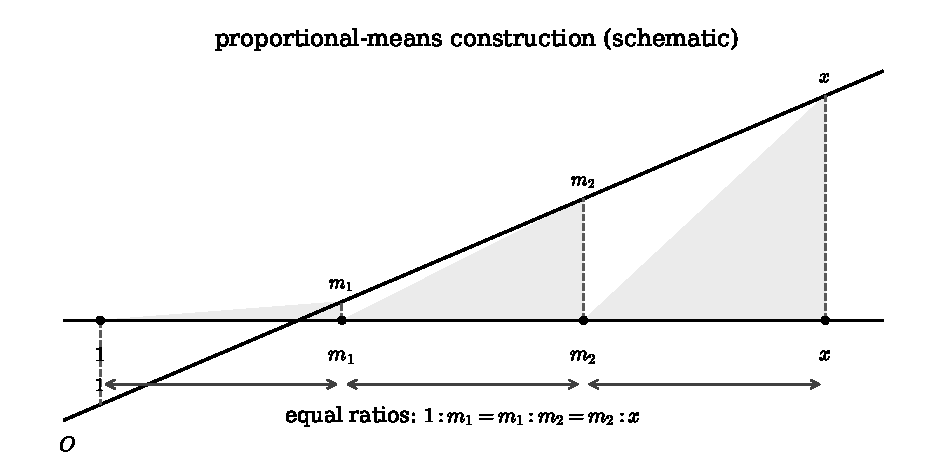
\includegraphics[width=0.86\linewidth]{../figures/fig1_pandrosion_construction.pdf}
  \caption{Proportional-means construction, with lengths not drawn to scale.  The dashed parallels encode the Thales-type step, and the shaded triangles indicate the repeated similarity condition $1:m_1=m_1:m_2=m_2:x$.}
  \label{fig:pandrosion-construction}
\end{figure}

Pandrosion's geometric procedure does not produce the exact value in finitely
many steps.  It produces a sequence of approximations.  This is the key modern
viewpoint: the construction is an iteration, and the error sequence of that
iteration is its residual profile.

In the classical cube-root case one may write the construction with an internal
length $u_n$ and a visible readout $v_n$:
\begin{equation}
  u_{n+1}
  =\frac{u_n}{2-2\left(\frac{4-u_n}{4}\right)^3},
  \qquad
  v_n=2\left(\frac{4-u_n}{4}\right)^2.
  \label{eq:classical-u}
\end{equation}
The number $u_n$ belongs to the diagram.  The number $v_n$ is the approximation
that is read from the diagram.

The substitution
\[
  s_n=\frac{4-u_n}{4}
\]
removes the distracting constants.  Since $u_n=4(1-s_n)$, the readout becomes
$v_n=2s_n^2$, and the iteration becomes
\begin{equation}
  s_{n+1}
  =\frac{2s_n^2+2s_n+1}{2s_n^2+2s_n+2}
  =1-\frac{1}{2(1+s_n+s_n^2)}.
  \label{eq:cube-s}
\end{equation}

\begin{proposition}[Cube-root fixed point]
The map in~\eqref{eq:cube-s} has the fixed point
\[
  s_*=2^{-1/3}.
\]
Consequently the readout satisfies
\[
  v_n=2s_n^2 \longrightarrow 2s_*^2=\cbrt{2}.
\]
\end{proposition}

\begin{proof}
The fixed-point equation is
\[
  s=1-\frac{1}{2(1+s+s^2)}.
\]
Multiplying by $2(1+s+s^2)$ gives
\[
  2s(1+s+s^2)=2(1+s+s^2)-1,
\]
which simplifies to $2s^3=1$.  Hence $s=2^{-1/3}$ in the positive real branch.
The readout identity follows immediately.
\end{proof}

\begin{takeaway}
The diagram computes $\cbrt{2}$ indirectly.  It first converges to
$2^{-1/3}$, and the visible root is recovered by the readout $v=2s^2$.
\end{takeaway}

%=====================================================================
\section{Why the polynomial \texorpdfstring{$S_p$}{Sp} appears}
\label{sec:geometry}
%=====================================================================

The polynomial
\[
  \Sp(s)=1+s+\cdots+s^{p-1}
\]
appears for a geometric reason.  Thales' theorem constructs proportional
segments.  Repeating the construction builds a finite geometric progression of
ratios.  Algebraically that progression is exactly $\Sp$.

The elementary identity behind the construction is
\begin{equation}
  1-s^p=(1-s)(1+s+\cdots+s^{p-1})=(1-s)\Sp(s).
  \label{eq:telescopic-Sp}
\end{equation}
Thus, whenever a diagram compares $1$ and $s^p$ through successive proportional
segments, the denominator $\Sp(s)$ is the natural object that records the
accumulated proportional means.

This identity is the bridge between the geometric construction and the
fixed-point map.

%=====================================================================
\section{The universal real-line iteration}
\label{sec:general}
%=====================================================================

Let $p\ge 2$ and $x>0$.  Define
\begin{equation}
  \Sp(s)=\sum_{k=0}^{p-1}s^k,
  \qquad
  \hp(s)=1-\frac{x-1}{x\Sp(s)}.
  \label{eq:hp-def}
\end{equation}
The Pandrosion iteration is
\begin{equation}
  s_{n+1}=\hp(s_n).
  \label{eq:pandrosion-iteration}
\end{equation}
The desired root is not $s_n$ itself.  It is read from $s_n$ by
\begin{equation}
  v_n=x s_n^{p-1}.
  \label{eq:readout}
\end{equation}

\begin{theorem}[Fixed point and readout]
\label{thm:fixed-point}
Let $x>1$ and $p\ge 2$.  The map $\hp$ has the positive fixed point
\[
  s_*=x^{-1/p}.
\]
At this fixed point the readout is
\[
  x s_*^{p-1}=x^{1/p}.
\]
\end{theorem}

\begin{proof}
The fixed-point equation $s=\hp(s)$ is
\[
  1-s=\frac{x-1}{x\Sp(s)}.
\]
Using~\eqref{eq:telescopic-Sp}, this is equivalent to
\[
  x(1-s)\Sp(s)=x-1,
  \qquad\text{hence}\qquad
  x(1-s^p)=x-1.
\]
Therefore $xs^p=1$, so $s=x^{-1/p}$ in the positive branch.  The readout is
then $x(x^{-1/p})^{p-1}=x^{1/p}$.
\end{proof}

\begin{remark}
The map $\hp$ is derivative-free in its definition.  It is built from the
finite geometric sum $\Sp$, not from the derivative of $s^p-x$.
\end{remark}

%=====================================================================
\section{The contraction ratio}
\label{sec:lambda}
%=====================================================================

The speed of the raw Pandrosion iteration is governed by the derivative of
$\hp$ at the fixed point.  This derivative is not used to define the method; it
is used only to analyze the residual profile.

Let
\[
  \alpha=x^{1/p}.
\]
Then $s_*=\alpha^{-1}$.

\begin{theorem}[Closed-form contraction factor]
\label{thm:lambda}
For $x>1$ and $p\ge2$, the linear contraction factor of the Pandrosion
iteration at the fixed point is
\begin{equation}
  \lambda_{p,x}=\hp'(s_*)
  =\frac{(\alpha-1)\sum_{k=1}^{p-1}k\alpha^{p-1-k}}
         {\sum_{k=0}^{p-1}\alpha^k}.
  \label{eq:lambda}
\end{equation}
Equivalently, with $S_p(\alpha)=1+\alpha+\cdots+\alpha^{p-1}$,
\begin{equation}
  \lambda_{p,x}
  =1-\frac{p}{S_p(\alpha)}
  =\frac{\alpha^p-p\alpha+p-1}{\alpha^p-1},
  \label{eq:lambda-simplified}
\end{equation}
where the final quotient has removable value $0$ at $\alpha=1$.  In particular,
\[
  \lambda_{2,x}=\frac{\alpha-1}{\alpha+1},
  \qquad
  \lambda_{3,x}=\frac{(\alpha-1)(\alpha+2)}{\alpha^2+\alpha+1}.
\]
\end{theorem}

\begin{proof}
Differentiate~\eqref{eq:hp-def}:
\[
  \hp'(s)=\frac{x-1}{x}\frac{\Sp'(s)}{\Sp(s)^2}.
\]
Substitute $s=\alpha^{-1}$ and use
\[
  \Sp(\alpha^{-1})
  =\sum_{k=0}^{p-1}\alpha^{-k}
  =\alpha^{1-p}\sum_{k=0}^{p-1}\alpha^k.
\]
The same change of powers in $\Sp'(\alpha^{-1})$ yields~\eqref{eq:lambda}.
For the compact formula, telescope the numerator:
\[
  (\alpha-1)\sum_{k=1}^{p-1}k\alpha^{p-1-k}
  =\sum_{k=0}^{p-1}\alpha^k-p
  =S_p(\alpha)-p.
\]
Dividing by $S_p(\alpha)$ gives the first equality in~\eqref{eq:lambda-simplified};
the rational quotient follows from
$S_p(\alpha)=(\alpha^p-1)/(\alpha-1)$ for $\alpha\ne1$.
\end{proof}




For later chart selection it is useful to record an equivalent one-line form of
this multiplier.

\begin{proposition}[Strict monotonicity of the monomial multiplier]
\label{prop:lambda-monotone}
Fix $p\ge2$ and put $y=e^\delta\ge1$.  Then
\[
  \delta\longmapsto \lambda_{p,e^\delta}
\]
is continuous on $[0,\infty)$, strictly increasing on $(0,\infty)$, satisfies
$\lambda_{p,1}=0$, and tends to $1$ as $\delta\to\infty$.  Equivalently,
$y\mapsto\lambda_{p,y}$ is strictly increasing on $[1,\infty)$.
\end{proposition}

\begin{proof}
Let
\[
  \alpha=y^{1/p}=e^{\delta/p}.
\]
By the compact formula~\eqref{eq:lambda-simplified}, for $\alpha>1$,
\[
  \lambda_{p,y}
  =\frac{\alpha^p-p\alpha+p-1}{\alpha^p-1}.
\]
Differentiate that rational function with respect to $\alpha$:
\[
  \frac{\dd}{\dd\alpha}\lambda_{p,y}
  =\frac{p\bigl((p-1)\alpha^p-p\alpha^{p-1}+1\bigr)}
         {(\alpha^p-1)^2}.
\]
It remains only to check the sign of
\[
  g_p(\alpha)=(p-1)\alpha^p-p\alpha^{p-1}+1.
\]
We have $g_p(1)=0$ and
\[
  g_p'(\alpha)=p(p-1)\alpha^{p-2}(\alpha-1)>0
  \qquad(\alpha>1).
\]
Therefore $g_p(\alpha)>0$ for every $\alpha>1$, hence
$\lambda_{p,y}$ is strictly increasing in $\alpha$, and therefore also in
$y=\alpha^p$ and in $\delta=p\log\alpha$.  The endpoint value follows from the
removable limit in~\eqref{eq:lambda-simplified}, and the limit at infinity is
immediate from the leading terms.
\end{proof}

The formula immediately explains the qualitative behavior:

\begin{itemize}
  \item if $x$ is close to $1$, then $\lambda_{p,x}$ is small and the raw
  geometry converges quickly;
  \item if $x$ is large, then $\lambda_{p,x}$ approaches $1$ and the raw
  geometry converges slowly;
  \item increasing $p$ at fixed large target makes the unscaled construction
  more delicate.
\end{itemize}

\begin{proposition}[Large-$p$ limit at fixed target]
For fixed $x>1$,
\[
  \lim_{p\to\infty}\lambda_{p,x}
  =1-\frac{\log x}{x-1}.
\]
\end{proposition}

\begin{proof}
Put $L=\log x>0$, so that $\alpha=e^{L/p}$.  Use the compact formula
\[
  \lambda_{p,x}=1-\frac{p}{S_p(e^{L/p})}.
\]
The only limit needed is the Riemann sum
\[
  \frac{1}{p}S_p(e^{L/p})
  =\frac1p\sum_{k=0}^{p-1} e^{Lk/p}
  \longrightarrow \int_0^1 e^{Lt}\,\dd t
  =\frac{e^L-1}{L}
  =\frac{x-1}{\log x}.
\]
Therefore
\[
  \frac{p}{S_p(e^{L/p})}
  \longrightarrow
  \frac{\log x}{x-1},
\]
and the claimed limit follows.  This proof avoids any interchange of a growing
weighted numerator with an error term; it uses only the uniform continuity of
$t\mapsto e^{Lt}$ on $[0,1]$.
\end{proof}

\begin{takeaway}
The number $\lambda_{p,x}$ is the fingerprint of Pandrosion's residual
profile.  Scaling works because it changes $x$ before this fingerprint is
formed.
\end{takeaway}


\begin{figure}[tbp]
  \centering
  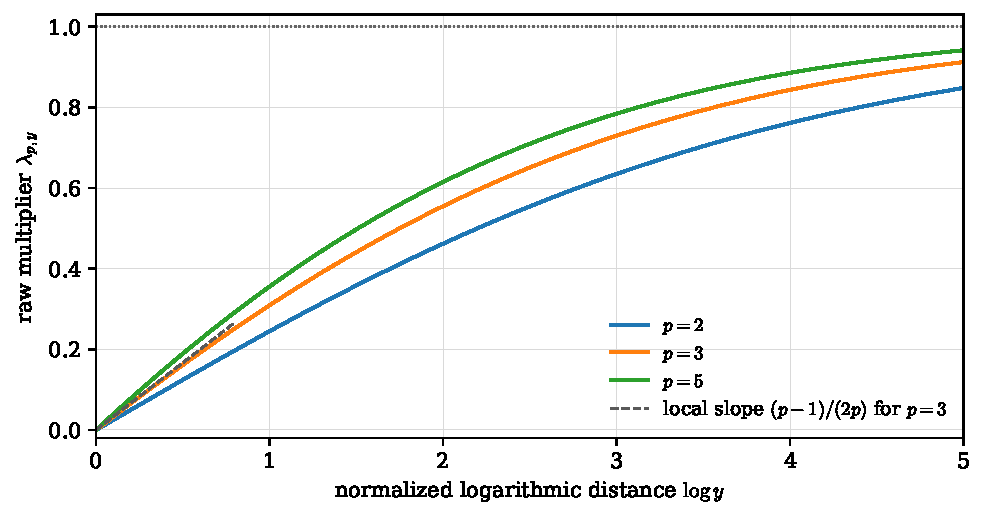
\includegraphics[width=0.86\linewidth]{../figures/fig2_lambda_profile.pdf}
  \caption{The residual fingerprint $\lambda_{p,y}$ as a function of the normalized logarithmic distance $\log y$.  The curves are monotone on the admissible branch $y\ge1$, and their initial slope is $(p-1)/(2p)$.}
  \label{fig:lambda-profile}
\end{figure}

\begin{remark}[Choosing a scale from a contraction threshold]
The simplified form~\eqref{eq:lambda-simplified} also gives an explicit scale
selection test.  Fix a desired raw multiplier $0<\tau<1$.  Since
$\lambda_{p,y}$ is continuous and strictly increasing on $y\ge1$, there is a
unique $\alpha_\tau>1$ satisfying
\[
  \frac{\alpha_\tau^p-p\alpha_\tau+p-1}{\alpha_\tau^p-1}=\tau.
\]
Thus every normalized target with
\[
  1\le y\le \alpha_\tau^p
\]
has raw multiplier at most $\tau$.  In a discrete scale family, one simply
chooses the available homothety whose normalized target lies closest to $1$;
Corollary~\ref{cor:log-chart-rule} below says that this also minimizes the
exact multiplier among the available admissible choices.
\end{remark}

%=====================================================================
\section{Error bounds and iteration counts}
\label{sec:bounds}
%=====================================================================

The local statement is the usual one for a contracting fixed-point map.  If an
interval $I$ contains $s_*$ and
\[
  \sup_{s\in I}|\hp'(s)|\le \Lambda<1,
\]
then every orbit that remains in $I$ satisfies
\begin{equation}
  |s_n-s_*|\le \Lambda^n |s_0-s_*|.
  \label{eq:basic-error}
\end{equation}
Consequently the readout error is controlled by the same geometric decay,
with an additional Lipschitz constant for $s\mapsto xs^{p-1}$ on $I$.

A practical iteration budget follows from~\eqref{eq:basic-error}.  To reach
$|s_n-s_*|\le \tau$, it is enough to take
\begin{equation}
  n\ge
  \frac{\log(\tau/|s_0-s_*|)}{\log \Lambda}.
  \label{eq:budget}
\end{equation}
The denominator is negative, so a smaller $\Lambda$ means a smaller budget.
This is the numerical meaning of the geometric statement: fewer effective
contractions are needed when the normalized multiplier is smaller.

%=====================================================================
\section{The case \texorpdfstring{$0<x<1$}{0 < x < 1}}
\label{sec:x-less-one}
%=====================================================================

When $0<x<1$, the fixed point
\[
  s_*=x^{-1/p}
\]
lies outside $(0,1)$.  This is not only a cosmetic inconvenience.  It changes
the real dynamics of the direct map.

Indeed, for every $s>0$ one has $S_p(s)>0$, and therefore
\[
  h_{p,x}(s)
  =1+\frac{1-x}{xS_p(s)}>1.
\]
Thus even if the diagram is initialized inside $(0,1)$, the next internal point
jumps outside that interval.  Moreover
\[
  h_{p,x}'(s)=\frac{x-1}{x}\frac{S_p'(s)}{S_p(s)^2}<0
  \qquad(s>0),
\]
so the map is orientation-reversing on the positive real line.  At the fixed
point, writing $\rho=s_*=x^{-1/p}>1$, the direct multiplier is
\begin{equation}
  h_{p,x}'(s_*)
  =-\mu_{p,x},
  \qquad
  \mu_{p,x}
  =\frac{(\rho-1)S_p'(\rho)}{S_p(\rho)}.
  \label{eq:direct-small-x-multiplier}
\end{equation}
This is not the same as the positive-target multiplier of $1/x$.  In fact,
as $x\to0^+$ one has $\rho\to\infty$ and
\[
  S_p(\rho)=\rho^{p-1}+O(\rho^{p-2}),
  \qquad
  S_p'(\rho)=(p-1)\rho^{p-2}+O(\rho^{p-3}),
\]
so
\[
  \mu_{p,x}
  =\frac{(\rho-1)S_p'(\rho)}{S_p(\rho)}
  \longrightarrow p-1.
\]
Hence for $p\ge3$ the direct chart is locally unstable for sufficiently small
$x$.  Even when the direct map happens to converge, it no longer has the same
clean ``nested proportional means inside a unit interval'' interpretation used
for $x>1$.

The canonical start also shows the scale problem clearly:
\[
  h_{p,x}(1)=1+\frac{1-x}{xp}.
\]
For very small $x$, this point is already very large.  In other words, the
direct affine chart asks the construction to travel to the far side of the
positive line before it can read the root.

The practical resolution is the reciprocal target.  Since
\[
  x^{1/p}=\frac{1}{(1/x)^{1/p}},
\]
one applies the $x>1$ theory to $1/x$ and then inverts the result.  This
restores the stable multiplier $\lambda_{p,1/x}<1$ from
Theorem~\ref{thm:lambda} instead of the direct orientation-reversing multiplier
\eqref{eq:direct-small-x-multiplier}.  In the reciprocal target $y=1/x>1$, the
internal fixed point is
\[
  s_y=y^{-1/p}=x^{1/p},
\]
which is already the desired root of the original target.  This is the first
appearance of a principle that becomes central later: changing charts is often
better than forcing one affine chart to handle every scale.

\begin{takeaway}
For $0<x<1$, direct Pandrosion is not algebraically wrong, but it is
geometrically misplaced.  The reciprocal chart restores the same positive-target
geometry while keeping the normalized fixed point near the intended root.
\end{takeaway}

%=====================================================================
\section{A better starting point}
\label{sec:start}
%=====================================================================

The raw iteration needs an initial point.  The most natural choice is not
always the fastest.  A simple geometric improvement is to start from the image
of the neutral point $1$:
\begin{equation}
  s_0^{\mathrm{opt}}=\hp(1)=1-\frac{x-1}{xp}.
  \label{eq:startopt}
\end{equation}
This point already incorporates one full proportional-mean step.  In the
language of the diagram, one avoids spending future parallels to do work that
can be done once at initialization.

\begin{proposition}[Canonical start]
The start $s_0^{\mathrm{opt}}=\hp(1)$ is the canonical one-step start produced
by the same Pandrosion geometry.  Near $x=1$ it satisfies
\[
  s_0^{\mathrm{opt}}=x^{-1/p}+O((x-1)^2).
\]
\end{proposition}

\begin{proof}
The first statement is the definition.  The expansion follows from
$x^{-1/p}=1-(x-1)/p+O((x-1)^2)$ and from
$1-(x-1)/(xp)=1-(x-1)/p+O((x-1)^2)$.
\end{proof}

Thus the canonical start removes the first-order local error of the neutral
start $s=1$.  Starting from $1$ gives
$s_*-1=-(x-1)/p+O((x-1)^2)$, whereas starting from $h_{p,x}(1)$ leaves only an
$O((x-1)^2)$ discrepancy.  This is the small but useful quantitative reason why
the numerical counts below always start from the canonical value.

\begin{takeaway}
Starting-point optimization is not an extra algorithmic layer.  It is the first
Pandrosion step used deliberately, before the iteration budget begins.
\end{takeaway}

%=====================================================================
\section{Steffensen acceleration}
\label{sec:steffensen}
%=====================================================================

The raw Pandrosion map is geometrically meaningful but only linearly
convergent.  Aitken--Steffensen acceleration turns any sufficiently regular
linearly convergent fixed-point iteration into a quadratically convergent one,
without requiring derivatives~\cite{aitken,steffensen,ostrowski}.

For $h=\hp$, define
\begin{equation}
  \stef(s)
  =s-\frac{(h(s)-s)^2}{h(h(s))-2h(s)+s}.
  \label{eq:steffensen}
\end{equation}

\begin{theorem}[Quadratic acceleration with explicit coefficient]
\label{thm:steffensen-explicit}
Assume $h$ is analytic near $s_*$, $h(s_*)=s_*$, and
\[
  \lambda=h'(s_*)\ne 1.
\]
Then the Steffensen map $\stef$ has a removable singularity at $s_*$, fixes
$s_*$, and satisfies
\begin{equation}
  \stef(s)-s_*
  =\frac{\lambda h''(s_*)}{2(\lambda-1)}(s-s_*)^2
  +O((s-s_*)^3).
  \label{eq:steffensen-constant}
\end{equation}
In particular, if $\lambda h''(s_*)\ne0$, the convergence is genuinely
quadratic.  If $\lambda=0$, or if $h''(s_*)=0$, the displayed quadratic coefficient
vanishes and the acceleration is at least quadratic, often of higher local order.
\end{theorem}

\begin{proof}
Write $e=s-s_*$ and expand
\[
  h(s_*+e)=s_*+\lambda e+a e^2+b e^3+O(e^4),
  \qquad a=\frac12h''(s_*).
\]
Then
\[
  h(s)-s=(\lambda-1)e+a e^2+b e^3+O(e^4).
\]
A second substitution gives
\[
  h(h(s_*+e))
  =s_*+\lambda^2 e+a\lambda(1+\lambda)e^2+O(e^3).
\]
Hence the denominator in \eqref{eq:steffensen} is
\[
  h(h(s))-2h(s)+s
  =(\lambda-1)^2e+a(\lambda-1)(\lambda+2)e^2+O(e^3).
\]
Since $\lambda\ne1$, this denominator has a simple zero at $e=0$ and the quotient
in \eqref{eq:steffensen} has a removable singularity.  Dividing the two series,
\[
  \frac{(h(s)-s)^2}{h(h(s))-2h(s)+s}
  =e-\frac{a\lambda}{\lambda-1}e^2+O(e^3).
\]
Therefore
\[
  \stef(s)-s_*
  =e-\left(e-\frac{a\lambda}{\lambda-1}e^2+O(e^3)\right)
  =\frac{a\lambda}{\lambda-1}e^2+O(e^3),
\]
which is \eqref{eq:steffensen-constant}.
\end{proof}

For the Pandrosion map itself,
\[
  h''_{p,x}(s)
  =\frac{x-1}{x}\,
    \frac{S_p''(s)S_p(s)-2(S_p'(s))^2}{S_p(s)^3}.
\]
This second derivative is non-zero throughout the useful positive real regime
$x>1$.  Indeed, for $s>0$,
\begin{equation}
  2(S_p'(s))^2-S_p(s)S_p''(s)
  =p s^{p-2}\sum_{r=0}^{p-2}(r+1)(p-r-1)s^r>0.
  \label{eq:Sp-convex-reciprocal}
\end{equation}
For completeness, here is the coefficient check.  Write $N=p-1$.  The
coefficient of $s^m$ in $2(S_p')^2-S_pS_p''$ is $0$ for $0\le m<N-1$, because
\[
2\sum_{i=1}^{m+1} i(m+2-i)-\sum_{i=2}^{m+2}i(i-1)=0.
\]
For $m=N-1+r$, $0\le r\le N-1$, the same coefficient is
\[
  2\sum_{i=r+1}^{N}i(N+1+r-i)-\sum_{i=\max(2,r+1)}^{N}i(i-1)
  =(N+1)(r+1)(N-r),
\]
which is exactly the coefficient of the right-hand side of
\eqref{eq:Sp-convex-reciprocal}.  Thus the displayed identity is an elementary
finite-sum identity, not an additional analytic assumption.
Thus, when $x>1$,
\[
  h''_{p,x}(s)
  =-\frac{x-1}{x}\,
    \frac{2(S_p'(s))^2-S_p(s)S_p''(s)}{S_p(s)^3}<0.
\]
Combined with $0<\lambda_{p,x}<1$, this proves that Steffensen--Pandrosion is
genuinely quadratic for every $p\ge2$ and $x>1$.

Steffensen acceleration is especially natural here.  The underlying geometric
map remains derivative-free, and the acceleration uses only evaluations of the
same map.

%=====================================================================
\section{Thales scaling}
\label{sec:scaling}
%=====================================================================

Scaling is the most important practical improvement.  Suppose $x$ is large.
Instead of applying Pandrosion directly to $x$, write
\begin{equation}
  x=A x',
  \label{eq:scaling-factor}
\end{equation}
where $A$ is chosen so that $x'$ is close to $1$.  Then
\[
  x^{1/p}=A^{1/p}(x')^{1/p}.
\]
One computes $(x')^{1/p}$ by Pandrosion and multiplies back by $A^{1/p}$.

Equivalently, write $A=B^p$ and set $z=Bu$.  The equation $z^p=x$ becomes
\[
  u^p=\frac{x}{B^p}.
\]
Thus Thales scaling is a homothety in the root coordinate: the computation is
performed on the normalized target $x/B^p$, and the result is transported back
by the return map $u\mapsto Bu$.

The point is not cosmetic.  The contraction factor is controlled by the
normalized target, not by the original target.  Since $\lambda_{p,x}$ becomes
small when $x$ is close to $1$, the scaled problem may require far fewer
effective Thales constructions.

\begin{takeaway}
Homothety does not merely normalize the input.  It changes the geometry before
Pandrosion begins.  A good homothety reduces the number of proportional layers
the construction must build.
\end{takeaway}

This is the one-dimensional ancestor of the chart-scaled construction developed
next.  Thales scaling normalizes the size of the problem inside one fixed
affine chart.  But a fixed chart may be the wrong place to measure the problem:
near $0$, scaling alone is less natural than first moving the computation to
the reciprocal chart.  The next step is therefore not a new iteration, but the
same homothetic idea after a change of chart.

%=====================================================================
\section{Geometric inversion}
\label{sec:geometric-inversion}
%=====================================================================

The reciprocal trick in Section~\ref{sec:x-less-one} and the homothety of
Section~\ref{sec:scaling} are two faces of the same geometric principle:

\begin{quote}
\emph{choose a chart, normalize by homothety, run Pandrosion near the fixed
point $1$, and transport the answer back.}
\end{quote}

The reciprocal trick is not merely an algebraic convenience; it is a change of
chart on the Riemann sphere
\[
  \widehat{\C}=\C\cup\{\infty\}.
\]
The inversion
\begin{equation}
  I(z)=\frac{1}{z}
  \label{eq:inversion-map}
\end{equation}
exchanges the neighborhoods of $0$ and $\infty$.  Thus a target $x$ that is
small in the usual affine chart becomes the large target $1/x$ in the reciprocal
chart.
\begin{figure}[tbp]
  \centering
  
\includegraphics[width=0.78\linewidth]{../figures/fig6_riemann_inversion.pdf}
  \caption{Direct and reciprocal logarithmic charts.  The affine chart uses $\log y_+(B)=\log x-p\log B$, while the reciprocal chart uses $\log y_\infty(B)=-\log x-p\log B$.  Chart selection chooses the line whose normalized logarithmic target lies closest to $0$.}
  \label{fig:riemann-inversion}
\end{figure}


For the equation
\[
  z^p=x,
\]
set $w=I(z)=1/z$.  Then
\begin{equation}
  w^p=\frac{1}{x}.
  \label{eq:inverted-root-equation}
\end{equation}
Therefore the root can be computed in the reciprocal coordinate and brought
back by another inversion:
\[
  z=\frac{1}{w}.
\]

This has a direct Pandrosion interpretation.  If $0<x<1$ and $y=1/x>1$, then
Pandrosion applied to $y$ has internal fixed point
\[
  s_y=y^{-1/p}=x^{1/p}.
\]
So, in the reciprocal chart, the fixed point itself is already the desired root
of the original target $x$.  If one uses the usual readout instead, one obtains
\[
  y s_y^{p-1}=y^{1/p}=x^{-1/p},
\]
and the final inversion gives $x^{1/p}$.

\begin{proposition}[Correctness of reciprocal Pandrosion]
Let $0<x<1$, $y=1/x$, and suppose the Pandrosion readout for $y$ converges to
$y^{1/p}$.  Then
\[
  \frac{1}{y^{1/p}}=x^{1/p}.
\]
Equivalently, the internal fixed point $s_y=y^{-1/p}$ is already equal to
$x^{1/p}$.
\end{proposition}

\begin{proof}
The first identity is immediate from $y=1/x$.  The second follows from
$s_y=y^{-1/p}=(1/x)^{-1/p}=x^{1/p}$.
\end{proof}

\begin{takeaway}
The interval $0<x<1$ is not a failure of Pandrosion.  It asks for a different
chart.  On the Riemann sphere, inversion moves the problem away from the small
scale near $0$ and into the same positive-target geometry used for $x>1$.
\end{takeaway}

%=====================================================================
\section{Inversion, homothety, and return of chart}
\label{sec:riemann-chart-scaling}
%=====================================================================

Inversion alone makes the interval $0<x<1$ compatible with the $x>1$ theory,
while Thales scaling makes large targets smaller.  The useful acceleration is to
combine both operations.  If $x$ is very small, then $1/x$ is very large, and the
contraction factor
$\lambda_{p,1/x}$ can be close to $1$.  The accelerated geometric idea is
therefore:

\begin{center}
\emph{invert, apply a homothety in the reciprocal chart, run Pandrosion near
$1$, and then return to the original chart.}
\end{center}

Let $B>0$ be a scale factor in the root coordinate.  There are two natural
charts.

\paragraph{Direct affine chart.}
Set
\[
  z=B u.
\]
Then $z^p=x$ is equivalent to
\begin{equation}
  u^p=y_+(B),
  \qquad
  y_+(B)=\frac{x}{B^p}.
  \label{eq:direct-chart-target}
\end{equation}
After computing $u\approx y_+(B)^{1/p}$, return
\[
  z\approx B u.
\]

\paragraph{Inverted chart.}
Set
\[
  z=\frac{1}{B u}.
\]
Then $z^p=x$ is equivalent to
\begin{equation}
  u^p=y_\infty(B),
  \qquad
  y_\infty(B)=\frac{1}{xB^p}.
  \label{eq:inverted-chart-target}
\end{equation}
After computing $u\approx y_\infty(B)^{1/p}$, return
\[
  z\approx \frac{1}{B u}.
\]

\begin{proposition}[Chart-scaled correctness]
Let $B>0$.
\begin{enumerate}
  \item If $u^p=x/B^p$, then $(Bu)^p=x$.
  \item If $u^p=1/(xB^p)$, then $(1/(Bu))^p=x$.
\end{enumerate}
Thus both the direct chart and the inverted chart solve the original equation
after their respective return maps.
\end{proposition}

\begin{proof}
The first identity gives $(Bu)^p=B^p u^p=B^p(x/B^p)=x$.  The second gives
\[
  \left(\frac{1}{Bu}\right)^p
  =\frac{1}{B^p u^p}
  =\frac{1}{B^p/(xB^p)}=x.
\]
\end{proof}

The speed is governed by the normalized target, not by the original target.  In
the direct chart the relevant contraction factor is
\[
  \lambda_{p,y_+(B)},
\]
whereas in the inverted chart it is
\[
  \lambda_{p,y_\infty(B)}.
\]
Thus one should choose the chart and the scale so that the normalized target is
as close to $1$ as possible.  This is why the logarithmic distance appears
below.  Since $|\log y|$ measures multiplicative distance from $1$, minimizing
it is a scale-invariant way to move the internal fixed point
$y^{-1/p}$ toward $1$.  By the contraction analysis of
Section~\ref{sec:lambda}, this is exactly the region where raw Pandrosion has
its smallest linear residual factor.  A concise selection rule is
\begin{equation}
  (\chi,B)\in
  \operatorname*{argmin}_{\chi\in\{+,\infty\},\,B\in\mathcal B}
  \left|\log y_\chi(B)\right|,
  \label{eq:chart-selection}
\end{equation}
with the admissibility constraint that the chosen normalized target lies in the
positive branch where the monotonicity theorem applies, namely $y_\chi(B)\ge 1$.
Here $\mathcal B$ is
the available family of homothetic scales: powers of $10$, powers of $2$, or
any constructible scale family allowed by the geometric model.

\begin{remark}
Equation~\eqref{eq:chart-selection} is the Riemann-sphere analogue of Thales
scaling.  Ordinary scaling chooses the size of the affine chart.  Riemann-chart
scaling also chooses whether the computation should be performed near $0$ or
near $\infty$.  Once that chart is selected, nothing else changes: the same
Pandrosion map is applied to the normalized target, and the return map carries
the result back to the original variable.
\end{remark}


\subsection{A local contraction lemma for chart selection}
\label{subsec:chart-contraction-lemma}

The rule \eqref{eq:chart-selection} can be justified directly from the closed
contraction formula.  In fact, Proposition~\ref{prop:lambda-monotone} proves
that, once the admissible normalized targets satisfy $y\ge1$, minimizing
$\log y$ is exactly the same thing as minimizing the raw linear multiplier
$\lambda_{p,y}$.  The local expansion below explains the first-order size of
that multiplier near the ideal target $1$.

Write a normalized positive target as
\[
  y=e^\delta,
  \qquad \delta=\log y.
\]
In the Pandrosion regime used here one usually arranges $y\ge 1$, so
$\delta\ge0$.  The ideal scaled target is $y=1$, for which the root in the
normalized coordinate is exactly $1$ and the residual geometry disappears.
The following expansion says that targets near $1$ have a contraction factor
proportional to their logarithmic distance from $1$.

\begin{lemma}[Local contraction factor near the normalized target]
\label{lem:local-chart-contraction}
For fixed $p\ge2$ and $y=e^\delta$ with $\delta\ge0$,
\[
  \lambda_{p,e^\delta}
  =\frac{p-1}{2p}\,\delta+O_p(\delta^2)
  \qquad(\delta\to0^+).
\]
Equivalently,
\[
  \lambda_{p,y}
  =\frac{p-1}{2p}\,\log y+O_p((\log y)^2)
  \qquad(y\to1^+).
\]
\end{lemma}

\begin{proof}
Put $\alpha=y^{1/p}=e^{\delta/p}$.  Uniformly for the finitely many exponents
that occur below,
\[
  \alpha^j=e^{j\delta/p}
  =1+\frac{j\delta}{p}+O_p(\delta^2),
  \qquad
  \alpha-1=\frac{\delta}{p}+O_p(\delta^2).
\]
Therefore
\[
  \sum_{k=0}^{p-1}\alpha^k
  =p+\frac{\delta}{p}\sum_{k=0}^{p-1}k+O_p(\delta^2)
  =p+\frac{p-1}{2}\delta+O_p(\delta^2),
\]
and
\[
  \sum_{k=1}^{p-1} k\alpha^{p-1-k}
  =\sum_{k=1}^{p-1}k
   +\frac{\delta}{p}\sum_{k=1}^{p-1}k(p-1-k)
   +O_p(\delta^2)
  =\frac{p(p-1)}{2}+O_p(\delta).
\]
Substituting these two estimates in \eqref{eq:lambda} gives
\[
  \lambda_{p,e^\delta}
  =\frac{\left(\frac{\delta}{p}+O_p(\delta^2)\right)
          \left(\frac{p(p-1)}{2}+O_p(\delta)\right)}
         {p+O_p(\delta)}
  =\frac{p-1}{2p}\delta+O_p(\delta^2),
\]
which is the announced expansion.
\end{proof}

\begin{corollary}[Exact logarithmic chart rule in the admissible regime]
\label{cor:log-chart-rule}
Let $\mathcal Y$ be any finite or infinite family of admissible normalized
targets with $y\ge1$.  For fixed $p\ge2$, a target $y_*\in\mathcal Y$ minimizes
$\log y$ over $\mathcal Y$ if and only if it minimizes the exact linear residual
factor $\lambda_{p,y}$ over $\mathcal Y$.

In particular, if the allowed homotheties form a discrete scale family, such as
powers of $2$ or powers of $10$, then the best available logarithmic
approximation to $1$ is also the best available choice for the raw Pandrosion
multiplier.
\end{corollary}

\begin{proof}
On the admissible branch $y\ge1$, $|\log y|=\log y$, and the logarithm is
strictly increasing in $y$.  Proposition~\ref{prop:lambda-monotone} says that
$\lambda_{p,y}$ is strictly increasing in the same variable.  Therefore the two
minimization problems have exactly the same minimizers.
\end{proof}

The same statement can be read directly in the scale parameter.  In the direct
chart,
\[
  \log y_+(B)=\log x-p\log B,
\]
whereas in the reciprocal chart,
\[
  \log y_\infty(B)=-\log x-p\log B.
\]
Thus chart selection asks for a scale $B$ whose logarithmic size best cancels
$\log x$ in whichever chart is being used.  If the scale family is discrete,
for example powers of $2$ or powers of $10$, the best available scale is the
nearest logarithmic approximation.  The monotonicity result above shows that
this is not merely a Taylor heuristic: within the admissible branch $y\ge1$, it
minimizes the exact raw multiplier among all available chart-scaled candidates.
This is the theoretical reason why the benchmark table below improves sharply:
the normalized target is moved from a large value to a value whose logarithmic
distance from $1$ is small.

\begin{theorem}[Tight two-chart scale-lattice bound]
\label{thm:q-lattice-two-chart}
Fix $p\ge2$ and a scale ratio $q>1$.  Let the available root-scales be the
$q$-lattice
\[
  \mathcal B_q=\{q^m:m\in\mathbb Z\}.
\]
For $x>0$, write $a=\log_q x$ and let
\[
  r=a-p\left\lfloor \frac{a}{p}\right\rfloor\in[0,p)
\]
be the remainder of $a$ modulo $p$.  In the direct chart, the best admissible
$q$-scale gives the normalized target $q^r$.  In the reciprocal chart, the best
admissible $q$-scale gives the normalized target $q^{p-r}$ when $r>0$, and $1$
when $r=0$.  Therefore the optimal two-chart target is
\[
  y_*(x)=q^{r_*},
  \qquad
  r_*=
  \begin{cases}
    0, & r=0,\\
    \min(r,p-r), & 0<r<p,
  \end{cases}
\]
and the optimal raw Pandrosion multiplier among all admissible candidates is
\[
  \lambda_{p,y_*(x)}.
\]
In particular,
\begin{equation}
  \lambda_{p,y_*(x)}
  \le \lambda_{p,q^{p/2}}
  =1-\frac{p}{S_p(\sqrt q)}.
  \label{eq:q-lattice-two-chart-bound}
\end{equation}
The bound is sharp for this scale lattice and these two charts: equality is
attained by targets with $r=p/2$.
\end{theorem}

\begin{proof}
In the direct chart one has
\[
  \log_q y_+(q^m)=a-pm.
\]
The admissible condition $y_+(q^m)\ge1$ is $a-pm\ge0$, so the closest admissible
choice to $1$ is $m=\lfloor a/p\rfloor$, giving $y_+=q^r$.  Similarly, in the
reciprocal chart,
\[
  \log_q y_\infty(q^m)=-a-pm.
\]
The closest admissible choice is $m=\lfloor -a/p\rfloor$.  The corresponding
remainder is $0$ if $r=0$ and $p-r$ otherwise.  When $r=0$, the normalized
target is exactly $y_*=1$, and the removable value in
\eqref{eq:lambda-simplified} gives $\lambda_{p,1}=0$.  Hence the best
two-chart logarithmic distance is $r_*\log q$.

By Corollary~\ref{cor:log-chart-rule}, minimizing this logarithmic distance in
the admissible branch is exactly the same as minimizing the raw multiplier.
Since $0\le r_*\le p/2$, Proposition~\ref{prop:lambda-monotone} gives
\[
  \lambda_{p,q^{r_*}}\le \lambda_{p,q^{p/2}}.
\]
Finally, $q^{p/2}=(\sqrt q)^p$, so the compact formula
\eqref{eq:lambda-simplified} gives
\[
  \lambda_{p,q^{p/2}}=1-\frac{p}{S_p(\sqrt q)}.
\]
If $r=p/2$, the direct chart gives the remainder $p/2$, while the reciprocal
chart gives the complementary remainder $p-r=p/2$.  Thus the two possible
orientations meet at the same midpoint of the logarithmic cell.  No admissible
candidate in the two-chart $q$-lattice can have smaller logarithmic distance
than $(p/2)\log q$, and the same monotonicity then proves sharpness of the
multiplier bound.
\end{proof}

\begin{corollary}[Magnitude-free local iteration budget]
\label{cor:q-lattice-complexity}
Under the hypotheses of Theorem~\ref{thm:q-lattice-two-chart}, set
\[
  \Lambda_{p,q}^{(2)}=1-\frac{p}{S_p(\sqrt q)}.
\]
After optimal two-chart $q$-lattice scaling, the asymptotic raw Pandrosion
multiplier is bounded by $\Lambda_{p,q}^{(2)}$, independently of the magnitude
of $x$ for fixed $p$ and $q$.  Consequently, inside any local contraction
interval, reducing an internal error by a factor $R>1$ requires at most
\[
  \left\lceil \frac{\log R}{-\log \Lambda_{p,q}^{(2)}}\right\rceil
\]
raw updates, up to the usual local-constant enlargement from
Section~\ref{sec:bounds}.  This worst-case bound is tight for the chosen
$q$-lattice and the two charts.  If $\Lambda_{p,q}^{(2)}=0$, this means that the
normalized target is exactly $1$; equivalently, $x$ lies exactly on the selected
scale lattice, and the linearized residual disappears in one idealized step.
\end{corollary}

For comparison, direct scaling alone on the same $q$-lattice gives the sharp
worst-case multiplier
\[
  \lambda_{p,q^p}=1-\frac{p}{S_p(q)}.
\]
Thus the reciprocal chart halves the worst-case logarithmic lattice gap: direct
scaling has $0\le r<p$, while the two-chart rule has $0\le r_*\le p/2$.
The preceding theorem is the $K=1$ case of a sharper minimax statement.  It is
useful because it separates what belongs to the monomial multiplier from what
belongs to the logarithmic preconditioner itself.  The combined table below
records the direct-lattice bound and the optimal $K$-phase bounds in one place.


\begin{theorem}[Minimax optimality of logarithmic chart palettes]
\label{thm:minimax-palette}
Fix a logarithmic period $A=p\log q$ and let $K\ge1$.  Among all choices of
$K$ phase offsets on the circle $\R/A\mathbb Z$, the smallest possible
worst-case logarithmic gap is
\[
  \frac{A}{2K}.
\]
It is attained if and only if the phases are equally spaced modulo $A$.
Consequently, for monomial Pandrosion the sharp minimax raw multiplier for a
$K$-phase logarithmic palette is
\begin{equation}
  \lambda_{p,\exp(A/(2K))}
  =1-\frac{p}{S_p(q^{1/(2K)})}.
  \label{eq:K-palette-bound}
\end{equation}
\end{theorem}

\begin{proof}
Put the $K$ phase offsets on a circle of circumference $A$.  The $K$ gaps
between consecutive offsets have total length $A$, so some gap has length at
least $A/K$.  Its midpoint is at distance at least $A/(2K)$ from every offset.
This proves the lower bound.  If the offsets are equally spaced, every gap has
length $A/K$, hence every point of the circle lies within $A/(2K)$ of an
offset.  This proves optimality and equality.  Since $\lambda_{p,y}$ is
strictly increasing with $\log y$ on the admissible branch, the worst-case
multiplier is minimized by the same covering-radius minimization.  Finally,
$\exp(A/(2K))=q^{p/(2K)}=(q^{1/(2K)})^p$, so the compact formula
\eqref{eq:lambda-simplified} gives \eqref{eq:K-palette-bound}.
\end{proof}

\begin{remark}
The case $K=1$ is the original two-chart $q^{\mathbb Z}$ lattice.  Larger
$K$ corresponds to allowing a small finite list of precomputed offsets
$B=q^{m+j/K}$.  The theorem is mainly included to show that the logarithmic
chart rule is not only sharp for the basic lattice: it is minimax optimal among
finite periodic scale palettes.
\end{remark}


\begin{center}
\small
\setlength{\tabcolsep}{5pt}
\begin{tabular}{@{}rrrrrr@{}}
\toprule
$q$ & $p$ & direct & $K=1$ & $K=2$ & $K=4$ \\
\midrule
$10$ & $3$ & $0.972973$ & $0.788170$ & $0.494997$ & $0.270393$ \\
$10$ & $5$ & $0.999550$ & $0.965703$ & $0.768132$ & $0.481621$ \\
$2$ & $3$ & $0.571429$ & $0.320377$ & $0.167458$ & $0.085286$ \\
$2$ & $5$ & $0.838710$ & $0.555265$ & $0.313678$ & $0.165382$ \\
$1.25$ & $3$ & $0.213115$ & $0.109273$ & $0.055239$ & $0.027760$ \\
$1.25$ & $5$ & $0.390766$ & $0.209870$ & $0.108350$ & $0.054994$ \\
\bottomrule
\end{tabular}
\end{center}


\begin{figure}[tbp]
  \centering
  
\includegraphics[width=0.92\linewidth]{../figures/fig3_scale_lattice.pdf}
  \caption{The scale-lattice theorem in one picture.  For a logarithmic period $h=p\log q$, equally spaced $K$-phase palettes have covering radius $h/(2K)$, and no $K$-point palette can do better.}
  \label{fig:scale-lattice}
\end{figure}

The ``direct'' column is $1-p/S_p(q)$.  The columns $K=1,2,4$ display the
sharp minimax multipliers $1-p/S_p(q^{1/(2K)})$.  The $K=1$ column is exactly
the two-chart bound of Theorem~\ref{thm:q-lattice-two-chart}; the later columns
show how precomputed offsets shrink the optimal logarithmic covering radius.


\begin{takeaway}
Thales scaling and Riemann-chart scaling are not separate tricks.  Both are
instances of the same contraction principle: make $|\log y|$ small before the
Pandrosion map begins.  Locally,
$\lambda_{p,y}\sim ((p-1)/(2p))\log y$; globally on $y\ge1$, the exact
multiplier is strictly increasing with $\log y$.
\end{takeaway}

This logarithmic rule is the main conceptual novelty of the monomial account.
The inversion $z\mapsto1/z$ and the homothety $z\mapsto Bz$ are classical
operations, but the closed multiplier \eqref{eq:lambda} explains exactly why
one should combine them: they are preconditioners for the residual factor, not
post-processing tricks applied after convergence.

\paragraph{Numerical check.}
The following table was generated with high-precision Python arithmetic.  All
iterations are performed in the normalized chart named in the ``chart'' column
before the final return map.  In that column, \emph{recip.} means reciprocal
chart only, while \emph{recip.+scale} means reciprocal chart plus a homothety
by $B$ in the inverted root coordinate.  Each row stops when the returned value
has relative error at most $10^{-12}$ as an approximation to the normalized
root $y^{1/p}$.

The column ``raw'' counts unaccelerated Pandrosion updates after the canonical
start $s_0=h_{p,y}(1)$.  The column ``Steff.'' counts
Steffensen--Pandrosion updates from the same internal start.  The column
``Newton'' counts Newton updates for $u^p=y$, started from the same visible
canonical value
\[
  u_0=y\,h_{p,y}(1)^{p-1}.
\]
Thus the table reports both the Pandrosion phenomenon and the standard
numerical baseline in exactly the same normalized problem.

\begin{center}
\scriptsize
\resizebox{\linewidth}{!}{%
\begin{tabular}{@{}rllrrrrrrr@{}}
\toprule
$p$ & $x$ & chart & $B$ & normalized $y$ & $\lambda_{p,y}$ & raw & Steff. & Newton & raw/Steff. \\
\midrule
$3$ & $2\cdot10^{-3}$ & recip. & $1$ & $500$ & $0.958294558$ & $659$ & $7$ & $13$ & $94$ \\
$3$ & $2\cdot10^{-3}$ & recip.+scale & $5$ & $4$ & $0.412598948$ & $30$ & $3$ & $5$ & $10$ \\
$3$ & $2\cdot10^{-6}$ & recip. & $1$ & $500000$ & $0.999529779$ & $59506$ & $13$ & $24$ & $4577$ \\
$3$ & $2\cdot10^{-6}$ & recip.+scale & $50$ & $4$ & $0.412598948$ & $30$ & $3$ & $5$ & $10$ \\
$5$ & $1/(3\cdot4^5)$ & recip. & $1$ & $3072$ & $0.993515266$ & $4295$ & $9$ & $29$ & $477$ \\
$5$ & $1/(3\cdot4^5)$ & recip.+scale & $4$ & $3$ & $0.385672651$ & $28$ & $3$ & $6$ & $9.3$ \\
$5$ & $5\cdot10^{-6}$ & recip. & $1$ & $200000$ & $0.999737824$ & $106226$ & $13$ & $44$ & $8171$ \\
$5$ & $5\cdot10^{-6}$ & recip.+scale & $10$ & $2$ & $0.256508225$ & $19$ & $3$ & $5$ & $6.3$ \\
\bottomrule
\end{tabular}%
}
\end{center}


\begin{figure}[H]
  \centering
  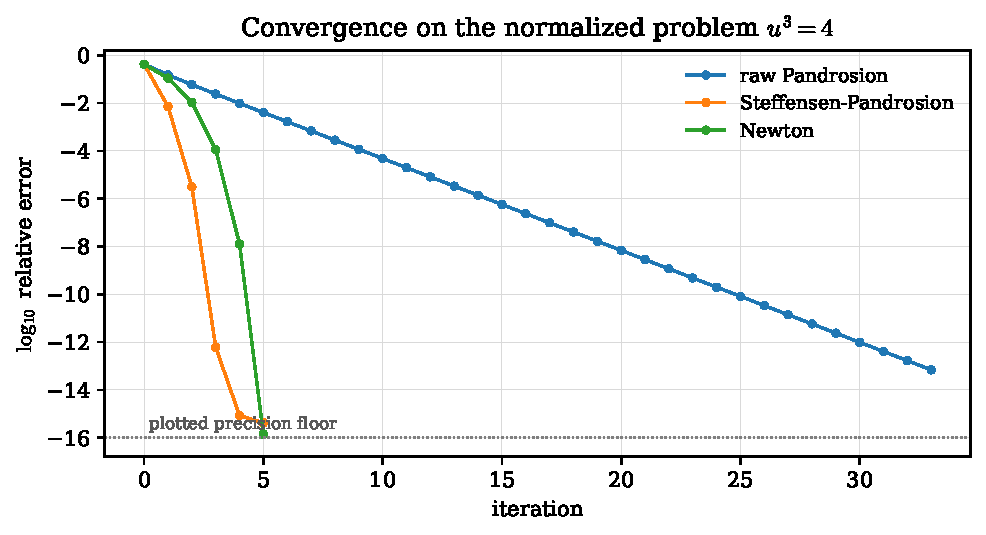
\includegraphics[width=0.86\linewidth]{../figures/fig4_convergence_comparison.pdf}
  \caption{Iteration histories on the normalized problem $u^3=4$.  Raw Pandrosion is linear, while Steffensen-Pandrosion and Newton show quadratic error collapse; the accelerated curves are truncated once they reach the plotted precision floor.}
  \label{fig:convergence-comparison}
\end{figure}

The Newton column clarifies the intended claim.  Newton is dramatically more
work-efficient than raw Pandrosion on the unscaled large targets, and it remains
a very strong baseline after scaling.  The Pandrosion-specific phenomenon is
not that it beats Newton as a production root extractor, but that the same
geometric map changes from nearly stalled to short and Steffensen-accelerable
once the reciprocal homothety makes $|\log y|$ small.

For example, when
$p=3$, $x=2\cdot10^{-6}$, and $B=50$, the inverted normalized target is
\[
  y_\infty(B)=\frac{1}{xB^p}
  =\frac{1}{(2\cdot10^{-6})50^3}=4.
\]
Pandrosion therefore works on the small target $4$ instead of the large target
$1/x=500000$, and the final answer is returned by
\[
  z=\frac{1}{50u}.
\]

\begin{takeaway}
Inversion is a chart change; homothety is a scale change inside that chart; the
return map transports the result back to the original variable.  The combined
procedure accelerates Pandrosion whenever it makes the normalized target closer
to $1$.
\end{takeaway}

%=====================================================================
\section{Comparison with standard methods}
\label{sec:comparison}
%=====================================================================

For $f(u)=u^p-x$, Newton's method can be written as
\begin{equation}
  u_{n+1}
  =u_n-\frac{u_n^p-x}{p u_n^{p-1}}
  =\frac{p-1}{p}u_n+\frac{x}{p u_n^{p-1}}.
  \label{eq:newton-monomial}
\end{equation}
This is quadratically convergent near a simple root and is very cheap for the
monomial problem: one power $u_n^{p-1}$, one division, and a few scalar
operations.  Halley's method and the higher Schröder--König families can have
even higher local order, at the price of using derivative information or more
structured rational formulas; see, for example, Schröder's classical papers~\cite{schroder1870,schroder1871} and the standard accounts~\cite{traub,householder}.

\paragraph{Relation with Schröder--König iterations.}
This comparison also sharpens the originality claim.  Standard Schröder--König
iterations are root-coordinate rational corrections built from $f$ and its
derivatives; for a simple root their multiplier at the root is zero when the
local order is at least two.  Raw Pandrosion has a different local signature.
Indeed, in a local branch of the readout map
\[
  r(s)=x s^{p-1},
\]
the induced root-coordinate map is $T=r\circ h\circ r^{-1}$, and therefore
\[
  T'(x^{1/p})=h'(s_*)=\lambda_{p,x}.
\]
For $x>1$ this multiplier is generally non-zero.  Hence the raw Pandrosion map
is not a disguised Newton, Halley, or fixed-order Schröder--König iteration
applied to $u^p-x$.  Steffensen acceleration later cancels this linear term,
but it does so by applying Aitken's $\Delta^2$ process to the Pandrosion
fixed-point map, not by replacing it with a derivative-based König formula.
This is the precise, limited novelty asserted here: a proportional-geometry map
with its own residual multiplier, plus chart scaling that controls that
multiplier.

Pandrosion is therefore not advertised here as a faster replacement for Newton
on ordinary monomial floating-point computation.  Its raw form is linearly
convergent, and its Steffensen form is quadratic but requires two evaluations of
the fixed-point map $h$ per accelerated update:
\[
  h(s),\qquad h(h(s)).
\]
Each evaluation of $h$ requires the finite geometric sum $S_p(s)$.  Evaluated by
Horner's rule, this sum costs $O(p)$ scalar operations and one division in the
formula for $h$.

A fair comparison must therefore separate convergence order from work per
update.  This is also the viewpoint behind the classical Kung--Traub efficiency
literature and modern derivative-free methods~\cite{kungtraub,petkovic2013,cordero2013,sharma2014}.

\begin{center}
\scriptsize
\begin{tabular}{@{}>{\raggedright\arraybackslash}p{0.20\linewidth}>{\raggedright\arraybackslash}p{0.10\linewidth}>{\raggedright\arraybackslash}p{0.36\linewidth}>{\raggedright\arraybackslash}p{0.16\linewidth}@{}}
\toprule
Method & Local order & Typical monomial work per update & Role here \\
\midrule
Raw Pandrosion & linear & $1$ evaluation of $S_p$ + $1$ division & geometric baseline \\
Steffensen--Pandrosion & quadratic & $2$ evaluations of $S_p$ + $2$ divisions & derivative-free acceleration \\
Newton & quadratic & $u^{p-1}$ + $1$ division & standard numerical baseline \\
Halley & cubic & derivatives/rational correction & higher-order baseline \\
\bottomrule
\end{tabular}
\end{center}

A crude cost-per-digit reading makes the comparison even sharper.  Evaluating
$S_p$ by Horner's rule costs $O(p)$ scalar operations, while the monomial power
$u^{p-1}$ in Newton costs $O(p)$ by a naive product and can be reduced to
$O(\log p)$ multiplications by binary exponentiation.  Conversely, away from
$s=1$, one may evaluate $S_p(s)$ through $(s^p-1)/(s-1)$, which gives a similar
fast-power route but introduces an additional division and a removable
singularity to handle near $s=1$.  Thus the scalar work model is already
favorable to Newton.  Even under the conservative convention that one evaluation
of $S_p$ and one monomial power evaluation are comparable $O(p)$ blocks, a
Newton update roughly doubles the number of correct digits
after one such block, whereas one Steffensen--Pandrosion update roughly doubles
the number of correct digits after two evaluations of $S_p$.  In this
asymptotic efficiency-index sense, Newton has effective index about $2$ per
monomial block, whereas Steffensen--Pandrosion has effective index about
$\sqrt2$ per $S_p$ block.  Halley is stronger still when its rational formula is
available.  This is only a crude scalar model, but it prevents the iteration
counts from being read as a speed claim.

The work-normalized message is thus modest.  For numerical root extraction of a
known monomial, Newton is usually the best default.  Pandrosion is interesting
for a different reason: it gives a proportional-geometry fixed-point operator
whose residual multiplier is exactly computable and whose chart-scaled
preconditioning is visible in closed form.

\paragraph{Where Pandrosion belongs.}
The natural niche of this paper is mathematical exposition, historical
reconstruction, and geometry-aware preconditioning.  The method is useful when
one wants to understand how a proportional-mean construction behaves as an
iteration, how homothety changes the residual factor, and how reciprocal charts
on the Riemann sphere can normalize small targets.  It is also a clean testing
ground for derivative-free acceleration because all constants are explicit.
The intended message is not that Pandrosion dominates Newton.  It usually does
not.  The message is that Pandrosion supplies a geometric fixed-point operator
whose residual profile is exactly analyzable and whose performance improves
substantially under chart scaling and Steffensen acceleration.

%=====================================================================
\section{Complex extension}
\label{sec:complex}
%=====================================================================

The real-line analysis identifies one positive fixed point.  Over $\C$, the
equation $s^p=1/x$ has $p$ fixed points:
\begin{equation}
  \gamma_k=x^{-1/p}\zeta_p^k,
  \qquad
  \zeta_p=e^{2\pi i/p},
  \qquad k=0,\dots,p-1.
  \label{eq:anchors}
\end{equation}
These are the cyclotomic anchors of the complex Pandrosion map.

\begin{figure}[tbp]
  \centering
  
\includegraphics[width=0.58\linewidth]{../figures/fig5_cyclotomic_anchors.pdf}
  \caption{Cyclotomic anchors for the complex monomial problem.  The poles are the non-trivial roots of unity; small disks around anchors provide local seeding regions for the accelerated map.}
  \label{fig:cyclotomic-anchors}
\end{figure}

The complex dynamics has non-trivial basin structure, as is typical for rational
iteration in one complex variable~\cite{milnor}.  A practical way to avoid
this difficulty is to seed points directly into a known local contraction disk
around the desired anchor.

\begin{definition}[Targeted seed]
Given an anchor $\gamma$ and a parameter $0<\eps<1$, define
\[
  \operatorname{seed}_{\gamma,\eps}(z)
  =\gamma+\eps(z-\gamma).
\]
\end{definition}

The seed is a homothety centered at $\gamma$.  It pulls any point $z$ closer to
the target anchor.  For $\eps$ small enough, the seeded point lies in a local
quadratic-convergence region for the Steffensen--Pandrosion map.


\begin{theorem}[Effective seeded complex convergence]
\label{thm:effective-seeded-complex}
Let $x\in\C\setminus\{0,1\}$ and let $\gamma$ be one of the anchors~\eqref{eq:anchors}.  Then
there exists an effectively computable radius $r_\gamma>0$ such that the
Steffensen--Pandrosion map is analytic on $D(\gamma,r_\gamma)$ after filling
its removable singularity at $\gamma$, fixes $\gamma$, and satisfies
\[
  |\stef(z)-\gamma|\le C_\gamma |z-\gamma|^2
  \qquad (z\in D(\gamma,r_\gamma))
\]
for some computable constant $C_\gamma$.  Consequently, every seeded point
$\operatorname{seed}_{\gamma,\eps}(z)$ with
\[
  |\operatorname{seed}_{\gamma,\eps}(z)-\gamma|<
  \min\left(r_\gamma,\frac{1}{2C_\gamma}\right)
\]
converges quadratically to $\gamma$ under Steffensen--Pandrosion.
\end{theorem}

\begin{proof}
The poles of $h_{p,x}$ are the zeros of $S_p$, namely the non-trivial
$p$-th roots of unity.  Since $x\ne1$, the anchor $\gamma$ is not one of these
poles.  Put
\[
  P_p=\{\omega:\omega^p=1,\ \omega\ne1\},
  \qquad
  d_0=\dist(\gamma,P_p)>0,
  \qquad
  R_0=d_0/4.
\]
Because $S_p(z)=\prod_{\omega\in P_p}(z-\omega)$, every
$z\in D(\gamma,R_0)$ satisfies
\[
  |S_p(z)|\ge (3d_0/4)^{p-1}.
\]
Together with the finite bounds
\[
  |S_p'(z)|\le\sum_{k=1}^{p-1}k(|\gamma|+R_0)^{k-1},
  \qquad
  |S_p''(z)|\le\sum_{k=2}^{p-1}k(k-1)(|\gamma|+R_0)^{k-2},
\]
this gives explicit bounds for $h$, $h'$, and $h''$ on $D(\gamma,R_0)$ from
the rational formula for $h$.  In particular one can choose a positive
$r_1\le R_0$ such that $h(D(\gamma,r_1))\subset D(\gamma,R_0)$.

Now set
\[
  D(z)=h(h(z))-2h(z)+z.
\]
The proof of Theorem~\ref{thm:steffensen-explicit} gives the local expansion
\[
  D(\gamma+e)=(\lambda-1)^2e+O(e^2),
  \qquad \lambda=h'(\gamma),
\]
and here $\lambda\ne1$.  Since all derivatives of $D$ on
$D(\gamma,r_1)$ are bounded effectively from the preceding rational bounds, one
can compute $B_\gamma$ with
\[
  |D(\gamma+e)-(\lambda-1)^2e|\le B_\gamma |e|^2
  \qquad(|e|\le r_1).
\]
Choose
\[
  r_2=\min\left(r_1,\frac{|\lambda-1|^2}{2B_\gamma}\right),
\]
with the evident convention $|\lambda-1|^2/(2B_\gamma)=+\infty$ when
$B_\gamma=0$.  Then $D(z)$ has no zero in $D(\gamma,r_2)\setminus\{\gamma\}$,
so the Steffensen quotient has only its removable singularity at $\gamma$.
On that disk, fill the singularity by Theorem~\ref{thm:steffensen-explicit} and
put
\[
  C_\gamma=
  \max_{|z-\gamma|=r_2}
  \left|\frac{\stef(z)-\gamma}{(z-\gamma)^2}\right|.
\]
This maximum is finite and computable to any prescribed precision because the
function is rational and pole-free on the circle.  The displayed quadratic
estimate follows from the maximum principle.  Finally, if
$|z_0-\gamma|<\min(r_2,1/(2C_\gamma))$, then
$|z_{n+1}-\gamma|\le C_\gamma |z_n-\gamma|^2$ keeps the orbit in the disk and
forces quadratic convergence.  Take $r_\gamma=r_2$.
\end{proof}

Once $\gamma_k$ is obtained, the corresponding root of $x$ is reconstructed by
\[
  \rho_k=x\gamma_k^{p-1}=x^{1/p}\zeta_p^{-k}.
\]
Thus the complex scheme is a multi-start method indexed by the cyclotomic
anchors.

%=====================================================================
\section{Selector regularity}
\label{sec:selector-regularity}
%=====================================================================

A target selector chooses which anchor should receive a starting point.  The
simplest selector is the nearest-anchor rule:
\begin{figure}[tbp]
  \centering
  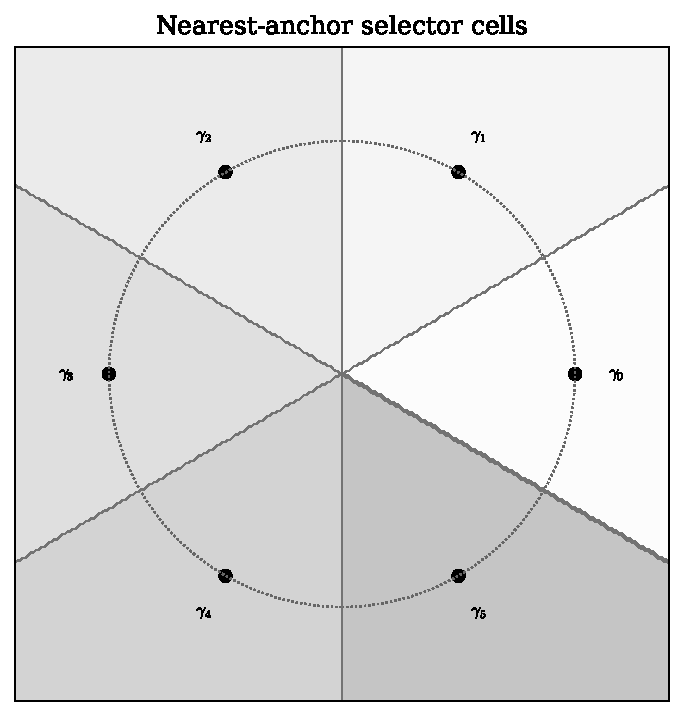
\includegraphics[width=0.58\linewidth]{../figures/fig7_anchor_voronoi.pdf}
  \caption{The nearest-anchor selector partitions the complex plane into Voronoi cells.  The selector is simple and locally stable away from the cell boundaries.}
  \label{fig:anchor-voronoi}
\end{figure}
 assign $z$ to the anchor
$\gamma_k$ that minimizes $|z-\gamma_k|$.

This is a finite Voronoi problem.  The boundaries between cells are finitely
many real line segments or rays determined by perpendicular bisectors of the
anchor set.  They have planar Lebesgue measure zero.  On the complement of
these boundaries, the selected anchor is locally constant.





\begin{proposition}[Piecewise regularity of the monomial selector]
The nearest-anchor selector is Borel measurable on $\C$ and locally constant
outside the Voronoi boundary.  On any compact set $K$ whose distance from the
boundary is at least $\eta>0$, the selected anchor is constant on every ball of
radius $\eta/2$ contained in $K$.  Consequently the seeded initial map
\[
  z\longmapsto \gamma+\eps(z-\gamma)
\]
is locally $\eps$-Lipschitz on each such cell, and every fixed finite number of
Steffensen--Pandrosion updates depends continuously on the input inside the
cell.
\end{proposition}

\begin{proof}
Voronoi cells are defined by finitely many inequalities
$|z-\gamma_k|\le |z-\gamma_j|$ between continuous functions, hence they are
Borel sets.  Their boundaries are contained in finitely many real affine lines,
so they have measure zero.  Away from the boundary, the nearest anchor does not
change under sufficiently small perturbations.  The seed map has Lipschitz
constant $\eps$, and the finite iterates are compositions of rational maps on a
pole-free neighborhood, hence are continuous there.
\end{proof}

This regularity statement is intentionally modest.  It is not a new
measure-theoretic theorem; it only records that the complex multi-start
construction has no hidden non-measurable selection step.

%=====================================================================
\section{Conclusion}
\label{sec:conclusion}
%=====================================================================

Pandrosion's construction can be read as a monomial root-finding algorithm.  In
modern notation, it is the fixed-point scheme
\[
  s_{n+1}=1-\frac{x-1}{x(1+s_n+\cdots+s_n^{p-1})}.
\]
Its fixed point is $x^{-1/p}$, its readout is $x^{1/p}$, and its contraction
ratio is the explicit quantity~\eqref{eq:lambda}.

The paper's originality is deliberately narrow.  It does not claim a new
all-purpose competitor to Newton.  It claims that the monomial Pandrosion
geometry admits a complete residual account organized by six facts:
\begin{enumerate}
  \item the finite geometric progression of proportional means forces the
  denominator $S_p$, and the multiplier is the closed form
  $1-p/S_p(\alpha)$;
  \item the same multiplier explains both Thales scaling and reciprocal
  Riemann-chart scaling;
  \item the logarithmic rule is local by the expansion
  $\lambda_{p,y}\sim ((p-1)/(2p))\log y$ and global on $y\ge1$ by
  monotonicity;
  \item on a $q$-lattice, the two-chart rule has the sharp
  magnitude-independent bound $1-p/S_p(\sqrt q)$, and $K$ equally spaced
  offsets are minimax optimal among $K$-phase palettes;
  \item raw Pandrosion is not a standard Schröder--König root-coordinate
  correction, because in root coordinates its derivative is
  $T'(x^{1/p})=\lambda_{p,x}\ne0$ for $x>1$;
  \item Steffensen acceleration preserves the derivative-free map while making
  the local convergence quadratic, and the complex monomial picture is handled
  by cyclotomic anchors and finite anchor selection.
\end{enumerate}

Thus the conceptual contribution is the chart-scaling principle, not raw speed:
before asking an iteration to converge, choose the chart in which its residual
factor is small.  In the Pandrosion viewpoint, homothety and inversion are not
post-processing tricks.  They are geometric preconditioners for the multiplier
of the fixed-point map.

The complex extension adds cyclotomic anchors, finite anchor selection, and
seeded local convergence.  This light version deliberately centers the monomial
equation $z^p=x$, because this is the setting where the finite geometric sum
$S_p$ gives a closed-form map and where the residual profile is fully explicit.
The elementary algebraic identities used here are suitable for a small
formal-audit companion, but no independent proof-assistant artifact is claimed
in this manuscript.

\section*{Acknowledgments}

\textbf{Generative AI disclosure.}
OpenAI Codex (GPT-5, accessed May 2026) was used during manuscript preparation
for LaTeX editing, anonymization, and editorial compliance checks.  The reason
for using the tool was to format the manuscript consistently, prepare an
anonymous submission version, and add the required disclosure statement.  The
author reviewed the AI-assisted output and remains responsible for the accuracy,
originality, integrity, and references of the manuscript.

%=====================================================================
\begin{thebibliography}{20}

\bibitem{pappus}
Pappus of Alexandria,
\textit{Collectio}, Book III, ca. 340 AD.
Critical edition: F. Hultsch, \textit{Pappi Alexandrini Collectionis quae supersunt},
Weidmann, Berlin, 1876--1878.

\bibitem{mactutor_pandrosion}
J. J. O'Connor and E. F. Robertson,
``Pandrosion of Alexandria,''
\textit{MacTutor History of Mathematics}, University of St Andrews, 2020.

\bibitem{mactutor_cube}
J. J. O'Connor and E. F. Robertson,
``Doubling the cube,''
\textit{MacTutor History of Mathematics}, University of St Andrews, 2002.

\bibitem{steffensen}
J. F. Steffensen,
``Remarks on iteration,''
\textit{Skandinavisk Aktuarietidskrift} \textbf{16} (1933), 64--72.

\bibitem{aitken}
A. C. Aitken,
``On Bernoulli's numerical solution of algebraic equations,''
\textit{Proceedings of the Royal Society of Edinburgh} \textbf{46} (1926), 289--305.

\bibitem{ostrowski}
A. M. Ostrowski,
\textit{Solution of Equations and Systems of Equations},
2nd ed., Academic Press, 1966.

\bibitem{traub}
J. F. Traub,
\textit{Iterative Methods for the Solution of Equations},
Prentice-Hall, 1964.

\bibitem{householder}
A. S. Householder,
\textit{The Numerical Treatment of a Single Nonlinear Equation},
McGraw-Hill, 1970.

\bibitem{schroder1870}
E. Schr\"oder,
``Ueber unendlich viele Algorithmen zur Aufl\"osung der Gleichungen,''
\textit{Mathematische Annalen} \textbf{2} (1870), 317--365.

\bibitem{schroder1871}
E. Schr\"oder,
``Ueber iterirte Functionen,''
\textit{Mathematische Annalen} \textbf{3} (1871), 296--322.

\bibitem{kungtraub}
H. T. Kung and J. F. Traub,
``Optimal order of one-point and multipoint iteration,''
\textit{Journal of the ACM} \textbf{21} (1974), 643--651.

\bibitem{petkovic2013}
M. S. Petkovi\'c, B. Neta, L. D. Petkovi\'c, and J. D\v{z}uni\'c,
\textit{Multipoint Methods for Solving Nonlinear Equations},
Academic Press, 2013.

\bibitem{cordero2013}
A. Cordero, J. L. Hueso, E. Mart\'inez, and J. R. Torregrosa,
``A new technique to obtain derivative-free optimal iterative methods for solving nonlinear equations,''
\textit{Journal of Computational and Applied Mathematics} \textbf{252} (2013), 95--102.

\bibitem{sharma2014}
J. R. Sharma, H. Arora, and M. S. Petkovi\'c,
``An efficient derivative free family of fourth order methods for solving systems of nonlinear equations,''
\textit{Applied Mathematics and Computation} \textbf{235} (2014), 383--393.

\bibitem{milnor}
J. Milnor,
\textit{Dynamics in One Complex Variable},
3rd ed., Princeton University Press, 2006.

\bibitem{henrici}
P. Henrici,
\textit{Applied and Computational Complex Analysis},
Wiley, New York, 1974--1986.

\end{thebibliography}

\end{document}
